%%%%%%%%%%%%%%%%%%%%%%%%%%%%%%%%%%%%%%%%%
% Masters/Doctoral Thesis
% LaTeX Template
% Version 2.5 (27/8/17)
%
% This template was downloaded from:
% http://www.LaTeXTemplates.com
%
% Version 2.x major modifications by:
% Vel (vel@latextemplates.com)
%
% This template is based on a template by:
% Steve Gunn (http://users.ecs.soton.ac.uk/srg/softwaretools/document/templates/)
% Sunil Patel (http://www.sunilpatel.co.uk/thesis-template/)
%
% Template license:
% CC BY-NC-SA 3.0 (http://creativecommons.org/licenses/by-nc-sa/3.0/)
%
%%%%%%%%%%%%%%%%%%%%%%%%%%%%%%%%%%%%%%%%%

%----------------------------------------------------------------------------------------
%	PACKAGES AND OTHER DOCUMENT CONFIGURATIONS
%----------------------------------------------------------------------------------------

% Pages (from the internal page numbering) to be printed in color - 3, 4, 5, 11, 12, 13, 14, 17, 18, 20, 21, 23, 25, 27.

\documentclass[
hidelinks,
12pt, % The default document font size, options: 10pt, 11pt, 12pt
oneside, % Two side (alternating margins) for binding by default, uncomment to switch to one side
english, % ngerman for German
doublespacing, % Single line spacing, alternatives: onehalfspacing or doublespacing
%draft, % Uncomment to enable draft mode (no pictures, no links, overfull hboxes indicated)
%nolistspacing, % If the document is onehalfspacing or doublespacing, uncomment this to set spacing in lists to single
%liststotoc, % Uncomment to add the list of figures/tables/etc to the table of contents
%toctotoc, % Uncomment to add the main table of contents to the table of contents
%parskip, % Uncomment to add space between paragraphs
%nohyperref, % Uncomment to not load the hyperref package
headsepline, % Uncomment to get a line under the header
%chapterinoneline, % Uncomment to place the chapter title next to the number on one line
%consistentlayout, % Uncomment to change the layout of the declaration, abstract and acknowledgements pages to match the default layout
]{MastersDoctoralThesis} % The class file specifying the document structure

\usepackage[utf8]{inputenc} % Required for inputting international characters
\usepackage[T1]{fontenc} % Output font encoding for international characters
\usepackage{subcaption}
\usepackage{mathpazo} % Use the Palatino font by default
\usepackage{booktabs}
\usepackage{colortbl}
\usepackage[final]{pdfpages}
\usepackage{xcolor}
\usepackage{balance}
\usepackage{epigraph}
\usepackage{alltt} % for code snippet
\usepackage{listings}
\usepackage{hyperref}
\usepackage{amsmath}
\usepackage[backend=bibtex,style=authoryear,natbib=true]{biblatex} % Use the bibtex backend with the authoryear citation style (which resembles APA)

\addbibresource{biblio.bib} % The filename of the bibliography


\usepackage[autostyle=true]{csquotes} % Required to generate language-dependent quotes in the bibliography

%----------------------------------------------------------------------------------------
%	MARGIN SETTINGS
%----------------------------------------------------------------------------------------

\geometry{
	paper=a4paper, % Change to letterpaper for US letter
	inner=4.0cm, % Inner margin
	outer=3.0cm, % Outer margin
	bindingoffset=.5cm, % Binding offset
	top=1.5cm, % Top margin
	bottom=1.5cm, % Bottom margin
	%showframe, % Uncomment to show how the type block is set on the page
}

%----------------------------------------------------------------------------------------
%	THESIS INFORMATION
%----------------------------------------------------------------------------------------

\thesistitle{Title of your Capstone} % Your thesis title, this is used in the title and abstract, print it elsewhere with \ttitle
\supervisor{Dr/Pr. FirstName \textsc{LastName}} % Your supervisor's name, this is used in the title page, print it elsewhere with \supname
\examiner{Dr/Pr. FirstName \textsc{LastName}} % Your examiner's name, this is not currently used anywhere in the template, print it elsewhere with \examname
\degree{B.Sc (Hons)} % Your degree name, this is used in the title page and abstract, print it elsewhere with \degreename
\author{FirstName \textsc{LastName}} % Your name, this is used in the title page and abstract, print it elsewhere with \authorname
\addresses{} % Your address, this is not currently used anywhere in the template, print it elsewhere with \addressname

\subject{Mathematical, Computational and Statistical Sciences} % Your subject area, this is not currently used anywhere in the template, print it elsewhere with \subjectname
\keywords{Insert, keywords, here} % Keywords for your thesis, this is not currently used anywhere in the template, print it elsewhere with \keywordnames
\university{\href{https://www.yale-nus.edu.sg/}{Yale-NUS College}} % Your university's name and URL, this is used in the title page and abstract, print it elsewhere with \univname
\department{{}} % Your department's name and URL, this is used in the title page and abstract, print it elsewhere with \deptname
\group{{}} % Your research group's name and URL, this is used in the title page, print it elsewhere with \groupname
\faculty{{}} % Your faculty's name and URL, this is used in the title page and abstract, print it elsewhere with \facname

\AtBeginDocument{
\hypersetup{colorlinks=false}
\hypersetup{pdftitle=\ttitle} % Set the PDF's title to your title
\hypersetup{pdfauthor=\authorname} % Set the PDF's author to your name
\hypersetup{pdfkeywords=\keywordnames} % Set the PDF's keywords to your keywords
}

\begin{document}

\frontmatter % Use roman page numbering style (i, ii, iii, iv...) for the pre-content pages

\pagestyle{plain} % Default to the plain heading style until the thesis style is called for the body content

%----------------------------------------------------------------------------------------
%	TITLE PAGE
%----------------------------------------------------------------------------------------

\begin{titlepage}
\begin{center}

\vspace*{.06\textheight}
{\scshape\LARGE \univname\par}\vspace{1.5cm} % University name
\textsc{\Large Capstone Report}\\[0.5cm] % Thesis type

\HRule \\[0.4cm] % Horizontal line
{\huge \bfseries \ttitle\par}\vspace{0.4cm} % Thesis title
\HRule \\[1.5cm] % Horizontal line

\begin{minipage}[t]{0.4\textwidth}
\begin{flushleft} \large
\emph{Author:}\\
{\authorname} % Author name - remove the \href bracket to remove the link
\end{flushleft}
\end{minipage}
\begin{minipage}[t]{0.4\textwidth}
\begin{flushright} \large
\emph{Supervisor:} \\
{\supname} % Supervisor name - remove the \href bracket to remove the link
\end{flushright}
\end{minipage}\\[3cm]

\vfill

\large \textit{A thesis submitted in fulfillment of the requirements\\ for the degree of \degreename}\\[0.3cm] % University requirement text
% \textit{in the}\\[0.4cm]
% \groupname\\\deptname\\[2cm] % Research group name and department name

\vfill

{\large \today}\\[4cm] % Date
%\includegraphics{Logo} % University/department logo - uncomment to place it

\vfill
\end{center}
\end{titlepage}

%----------------------------------------------------------------------------------------
%	DECLARATION & CONSENT
%----------------------------------------------------------------------------------------

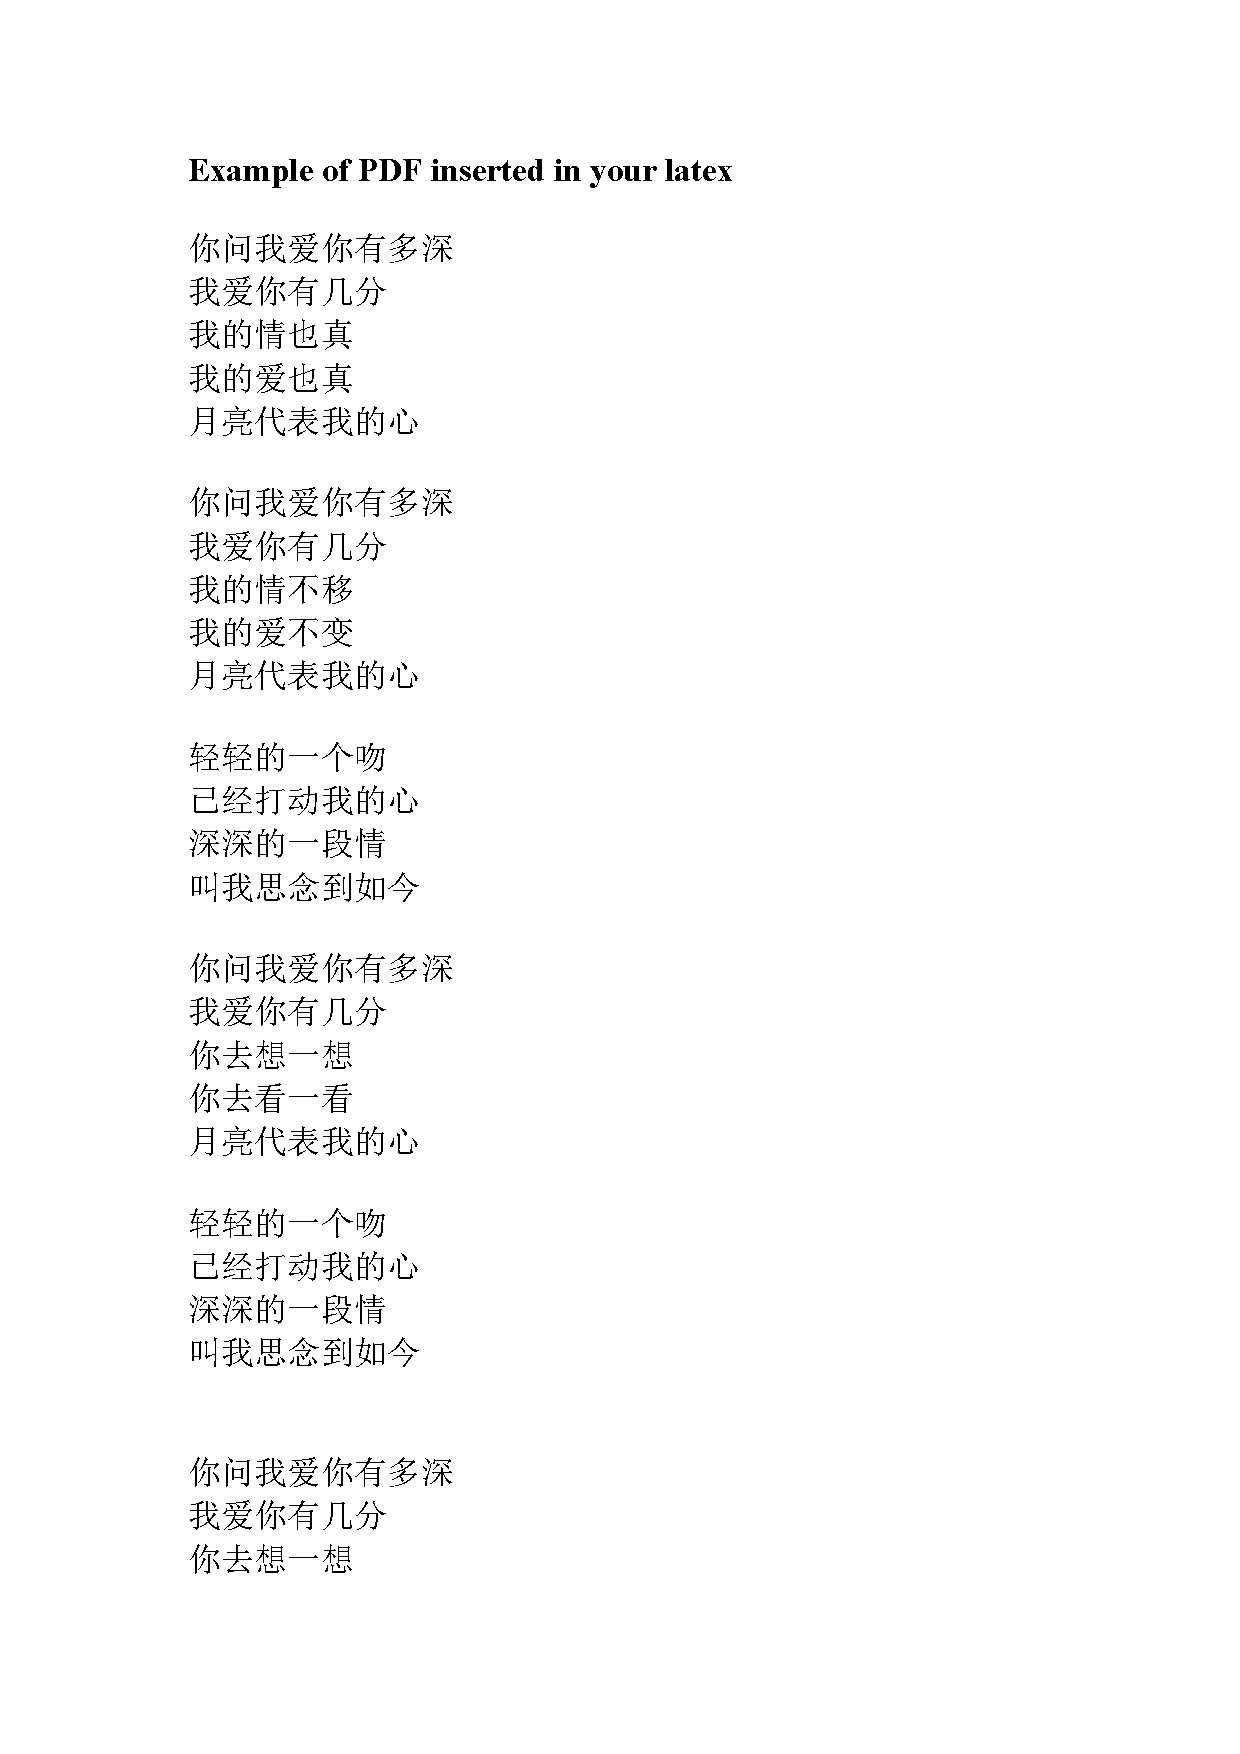
\includepdf[pages=-,pagecommand={},width=\textwidth]{pdfexample.pdf}

%----------------------------------------------------------------------------------------
%	ACKNOWLEDGEMENTS
%----------------------------------------------------------------------------------------

\begin{acknowledgements}
\addchaptertocentry{\acknowledgementname} % Add the acknowledgements to the table of contents
Acknowledgements go here.
\end{acknowledgements}

%----------------------------------------------------------------------------------------
%	ABSTRACT PAGE
%----------------------------------------------------------------------------------------

\begin{abstract}
\addchaptertocentry{\abstractname} % Add the abstract to the table of contents
Abstract goes here.
\end{abstract}


%----------------------------------------------------------------------------------------
% CONTRIBUTIONS
%----------------------------------------------------------------------------------------

% \chapter{Claims}
%
% This paper presents the following original contributions:
%
% \begin{enumerate}
% 	\item A hardware device for haptic sensory substitution along with designs for the construction of such a system.
% 	\item Two implementations of sensory substitution using haptic feedback, continuous and delayed feedback-based spatial navigation tasks, each of which include:
% 		\begin{enumerate}
% 			\item a front-end for providing visual input to the user during the training phase with useful readouts to the researcher,
% 			\item a transmission protocol, which maps information from the task at hand (spatial coordinates, velocity information, etc) to time-based sensor actuation signals (20$^{\circ}$ on servo 1, 35$^{\circ}$ on servo 2, etc) in real-time.
% 		\end{enumerate}
% 	\item An evaluation framework for measuring the performance of a sensory substitution system, which provides sample tasks that can be used to standardise and compare performance across the board for future research.
% 	\item A review of existing hardware and software stacks as well as possible avenues for development based on the developed metrics.
% \end{enumerate}
%
% In addition, code for displaying results in real-time, modules for managing servo overload, network latency and other factors were also written by the author.


% %----------------------------------------------------------------------------------------
% %	DECLARATION PAGE
% %----------------------------------------------------------------------------------------
%
% \begin{declaration}
% \addchaptertocentry{\authorshipname} % Add the declaration to the table of contents
%
% \noindent I, \authorname, hereby declare that this Project, the Capstone Report and associated work listed herein, is the end result of my own work and that due acknowledgement has been given in the bibliography and references to ALL sources printed, electronic, or personal, in accordance with the academic regulations of Yale‐NUS College.
% I acknowledge that the Thesis is subject to the policies relating to Yale‐NUS College Intellectual  Property (Yale‐NUS HR 039).
%
%
% % I confirm that:
% %
% % \begin{itemize}
% % \item This work was done wholly or mainly while in candidature for a research degree at this University.
% % \item Where any part of this thesis has previously been submitted for a degree or any other qualification at this University or any other institution, this has been clearly stated.
% % \item Where I have consulted the published work of others, this is always clearly attributed.
% % \item Where I have quoted from the work of others, the source is always given. With the exception of such quotations, this thesis is entirely my own work.
% % \item I have acknowledged all main sources of help.
% % \item Where the thesis is based on work done by myself jointly with others, I have made clear exactly what was done by others and what I have contributed myself.\\
% % \end{itemize}
%
% \noindent Signed:\\
% \rule[0.5em]{25em}{0.5pt} % This prints a line for the signature
%
% \noindent Date:\\
% \rule[0.5em]{25em}{0.5pt} % This prints a line to write the date
% \end{declaration}
%
% \cleardoublepage

%----------------------------------------------------------------------------------------
%	QUOTATION PAGE
%----------------------------------------------------------------------------------------

% \vspace*{0.2\textheight}
%
% \noindent\enquote{\itshape Thanks to my solid academic training, today I can write hundreds of words on virtually any topic without possessing a shred of information, which is how I got a good job in journalism.}\bigbreak
%
% \hfill Dave Barry

%----------------------------------------------------------------------------------------
%	LIST OF CONTENTS/FIGURES/TABLES PAGES
%----------------------------------------------------------------------------------------

\tableofcontents % Prints the main table of contents

\listoftables % Prints the list of tables
\label{lst:tabs}

\listoffigures % Prints the list of figures
\label{lst:figs}
%----------------------------------------------------------------------------------------
%	ABBREVIATIONS
%----------------------------------------------------------------------------------------

% \begin{abbreviations}{ll} % Include a list of abbreviations (a table of two columns)
%
% \textbf{LAH} & \textbf{L}ist \textbf{A}bbreviations \textbf{H}ere\\
% \textbf{WSF} & \textbf{W}hat (it) \textbf{S}tands \textbf{F}or\\
%
% \end{abbreviations}

%----------------------------------------------------------------------------------------
%	PHYSICAL CONSTANTS/OTHER DEFINITIONS
%----------------------------------------------------------------------------------------

% \begin{constants}{lr@{${}={}$}l} % The list of physical constants is a three column table
%
% % The \SI{}{} command is provided by the siunitx package, see its documentation for instructions on how to use it
%
% Speed of Light & $c_{0}$ & \SI{2.99792458e8}{\meter\per\second} (exact)\\
% %Constant Name & $Symbol$ & $Constant Value$ with units\\
%
% \end{constants}

%----------------------------------------------------------------------------------------
%	SYMBOLS
%----------------------------------------------------------------------------------------

% \begin{symbols}{lll} % Include a list of Symbols (a three column table)
%
% $a$ & distance & \si{\meter} \\
% $P$ & power & \si{\watt} (\si{\joule\per\second}) \\
% %Symbol & Name & Unit \\
%
% \addlinespace % Gap to separate the Roman symbols from the Greek
%
% $\omega$ & angular frequency & \si{\radian} \\
%
% \end{symbols}

%----------------------------------------------------------------------------------------
%	DEDICATION
%----------------------------------------------------------------------------------------

\dedicatory{Dedicated to ceux l\`{a} qui veulent.}

%----------------------------------------------------------------------------------------
%	THESIS CONTENT - CHAPTERS
%----------------------------------------------------------------------------------------

\mainmatter % Begin numeric (1,2,3...) page numbering

\pagestyle{thesis} % Return the page headers back to the "thesis" style

% Include the chapters of the thesis as separate files from the Chapters folder
% Uncomment the lines as you write the chapters

% Chapter 1

\chapter{Tips} % Main chapter title

\epigraph{``Y a plein de c\^otes \`a Ibiza\\C'est vraiment dur il fait tr\`es chaud.''}{\textit{Zambla}}

\label{chapter1} % For referencing the chapter elsewhere, use \ref{Chapter1}

%----------------------------------------------------------------------------------------
\section{Introduction}
Dear student reading that chapter, greetings!
After doing some research and writing reports for more than 12 years, I realized that LaTeX is the second worst way to write a thesis.
The worst one is Word.
Then you may be wondering, which is the best way to write a report?
Well, actually there is no best way.
Hence you are stuck with LaTeX.

\subsection{Goal of this chaper}
In this chapter, I will demonstrate a few interesting features of LaTeX, and more importantly, provide examples of Figures, Tables, Equations.
These may be easy to deal with on Word, but here it is another story.
The general idea is to keep these examples, copy-paste them, then modify them to fit your needs.
If you are seeing this content while reading \texttt{main.pdf}, please load the overall LaTeX project in your LaTeX editor, and open the \texttt{chapters/chaper1.tex}.
\\
\\
Done?
Ok let us move on then!
So by now, you should have noticed a few things:
\begin{itemize}
  \item Each sentence of the text is on a distinct line. Yet, sentences are still within the same paragraph.
  \item Backslash is an escape character, used at the beginning of LaTeX commands.
  \item To end a paragraph (or actually insert a newline), we can use the \textbackslash{}\textbackslash{} command.
\end{itemize}
Also now you know how to do a bullet list.

\subsection{Structure of a chapter}
Chapter contain sections (defined with \textbackslash{}section\{Name of your section\}), subsections (\textbackslash{}subsection).

\subsubsection{Because subsubsection that's why!}
Subsubsections are also available (\textbackslash{}subsubsection).

\paragraph{Paragraph}
If you really insist, there are also paragraphes, which may or may not be the same as a subsubsection.
Note that the automatically generated table of contents only goes to two levels of depth within chapters by default.
This can be changed, but you likely do not want to do that.

\subparagraph{Subparagraph}
I was today years old when I discovered the subparagraph. Seriously, do not use it.

\section{Font Formatting Commands}
Similarly to Word, LaTeX provides simple formatting, including \textbf{bold}, \textit{italic}, \underline{underlined} and \texttt{ugly stuff}.
However, no underline or strikethrough by default.
You can also change the size of the text, using {\tiny tiny}, {\small small}, {\large large}, {\huge huge}.
These last commands work within a specific scope.
The scope can be specified using \{ and \}, with the \{ placed before the \textbackslash{}size command.

\subsection{Special characters}
LaTeX uses 10 special characters. Each of these characters has a special meaning.
\begin{enumerate}
  \item Ampersand (\&) is used in tables as a cell delimiter.
  \item Percent sign (\%) is used for commenting a line.
  \item Dollar sign (\$) is used to switch back/from mathematical notation mode.
  \item Hash sign (\#) is used to create macros --- you definitely do not want to go more in depth here.
  \item Underscore (\_ or \textunderscore) is used to indicate a subscript in maths mode, if you use it in text mode ( without using backslash in front to ''escape'' it), your project will not compile anymore. \textbf{You may want to read that twice, and remember it.} It is in a LaTeX template, therefore it must be true.
  \item Curly brackets (\{ and \}) or bracets are used by LaTeX commands, as you likely already noticed.
  \item Tilde (\textasciitilde) can be used to create a non-breaking space (so that both words are on the same line).
  \item Caret/Circumflex/Hat (\textasciicircum) is used to indicate superscript (exponent) in maths mode.
  \item Backslash (\textbackslash) is used in front of every command. You cannot simply escape it to print it, as \textbackslash{}\textbackslash{} create a new line.
\end{enumerate}
If you happen to insert some of these symbols in your text without either escaping (when possible) or using the correct command, your project will likely not compile.
Thus, you may want to be extra careful about that problem.
Note: the underscore issue may also be encountered with bibliography.
So if \texttt{bibtex} displays an error, it may also come from an underscore somewhere in the abstract, DOI or URL field.

\section{Equations}
Here is an example of equation:
\begin{equation}
\int_0^\infty e^{-x^2} dx
\label{eq:eq1}
\end{equation}

I could also want to have this equation inline, i.e. within the text: $\int_0^\infty e^{-x^2} dx$.
In that case, simply use \textdollar{} (by the way, note that using the dollar sign in your text switches to mathematical notation. To actually print a dollar sign use the \textbackslash{}textdollar command).
The equation above has a label, meaning you can refer to it. The numbering system uses the chapter number (in this case 1), then the equation position within the chapter (1 again).
Example: Equation~\ref{eq:eq1} is an example of an equation in LaTeX{}.
In case you would like to have an equation without numbering it? Easy!
\begin{equation*}
t = a \times log_{2}(\frac{D}{W} + 1) + b
\end{equation*}

The only difference? Note the \textasteriskcentered symbol in the \textbackslash{}begin\{equation\textbf{\textasteriskcentered}\}.
This also works with Figures and Tables.

\section{Code Snippets}

\begin{lstlisting}
  int main (int argc, char ** argc)
  {
    printf("Hello world!\n");
    return 0;
  }
\end{lstlisting}

This package is not the best way to show code snippets.
However, many other packages you could use have compatibility issues.
Feel free to try alternatives, e.g. \texttt{minted}.

\section{Figures}
Figures are a bit tricky with LaTeX {\tiny(not as much as tables though)}.
Let us see a simple example below:
\begin{figure}[!h]
  \centering
    
\includegraphics[width=0.9\textwidth]{figures/future.png}
  \caption{When a YNC alumni tells you that back in their days, they did not have LaTeX template and would write their report in latin on a papyrus.}
  \label{fig:future}
\end{figure}
You can refer to it: Figure~\ref{fig:future}.
This is possible thanks to the \textbackslash{}label command.
The figure should also be shown on the \hyperref[lst:figs]{List of Figures} page (note this other way of referring to another part of the manuscript!).
A common practice is use the following naming convention:
\begin{itemize}
  \item A prefix, indicating the nature of the object labelled: \texttt{eq} for equation, \texttt{fig} for figure, \texttt{tab} for \texttt{table}.
  \item A colon.
  \item A unique name (easy to remember) describing your figure. Example: exp1confmatrix would suggest that the figure shows a confusion matrix for your experiment 1.
\end{itemize}

A few other points: The \textbackslash{}caption and \textbackslash{}label can be put either before or after the \textbackslash{}includegraphics command.
When you create a Figure, you need to provide placement information for LaTeX. LaTeX will usually not locate the figures \emph{exactly} where you want them.
The most common specifiers are: \texttt{h} (here), \texttt{b} (bottom of the page) and \texttt{t} (top). The \texttt{!} specifiers tries to force LaTeX to put the image exactly at the location you specified (with mixed success though).
For a longer list of specifiers, please refer to: \url{https://en.wikibooks.org/wiki/LaTeX/Floats,_Figures_and_Captions}.

\subsection{Figure Size}
The size of the figure can be determined by the first parameter of the \textbackslash{}includegraphics command.
In this example, we set the size to be $0.9 \times \texttt{textwidth}$, or 90\% of the size of a column.
We could have used an absolute value in cm, e.g. \texttt{width=19cm}.

\subsection{Supported Formats}
Use standard formats, such as PNG, PDF, JPG.
LaTeX also supports other formats, such as EPS.
\textbf{Rule of thumb: use PDF as much as you can, as it uses vector graphics, making it easy to scale the figure to very large format without problems.}

\subsection{Multiple images in one figure}
You can also create complex figures with multiple images.
Here is an example, which uses a $2\times2$ layout.
The overall figure can be referred as Figure~\ref{fig:drake}.
\begin{figure}[!h]
  \begin{subfigure}[t]{.5\textwidth}
    \centering
    
\includegraphics[width=\linewidth]{figures/draketl.png}
    %\caption{We could totally insert a caption here}
    %\label{fig:draketl}
  \end{subfigure}
  \hfill
  \begin{subfigure}[t]{.5\textwidth}
    \centering
    
\includegraphics[width=\linewidth]{figures/draketr.png}
    %\caption{We could totally insert a caption here}
        %\label{fig:draketr}
  \end{subfigure}

  %\medskip
  % the medskip will have white space between both lines
  \begin{subfigure}[t]{.5\textwidth}
    \centering
    
\includegraphics[width=\linewidth]{figures/drakebl}
    %\caption{We could totally insert a caption here}
        %\label{fig:drakebl}
  \end{subfigure}
  \hfill
  \begin{subfigure}[t]{.5\textwidth}
    \centering
    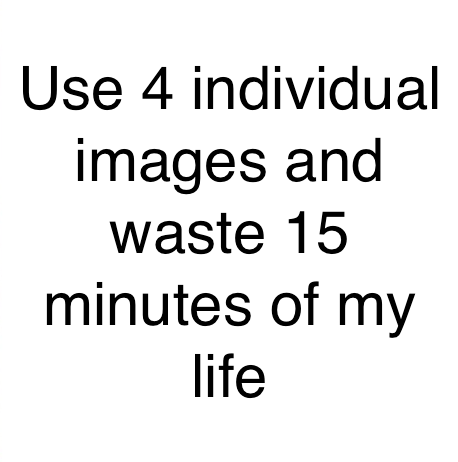
\includegraphics[width=\linewidth]{figures/drakebr}
    %\caption{We could totally insert a caption here}
    %\label{fig:drakebr}
  \end{subfigure}
  \caption{Example of a complex figures on a $2\times2$ layout.}
  \label{fig:drake}
\end{figure}

\section{Tables}
Tables can be a nightmare in LaTeX.
The easiest way to deal with tables in LaTeX is to use some online tools.
My favorite so far: \url{https://www.tablesgenerator.com/}

Here is an example of confusion matrix generated:
\begin{table}[!h]
  \resizebox{\textwidth}{!}{
\begin{tabular}{|c|c|ccccccccc}
\cline{1-2}
Chest (C)                         & -     &                                                                          &                                                                           &                                                                          &                          &                            &                           &                           &                            &                                                                            \\ \cline{1-3}
Chest (ND)  & *     & \multicolumn{1}{c|}{-}                                                   &                                                                           &                                                                          &                          &                            &                           &                           &                            &                                                                            \\ \cline{1-4}
Chest (D)   & *     & \multicolumn{1}{c|}{-}                                                   & \multicolumn{1}{c|}{*}                                                    &                                                                          &                          &                            &                           &                           &                            &                                                                            \\ \cline{1-5}
Ear          & -     & \multicolumn{1}{c|}{-}                                                   & \multicolumn{1}{c|}{-}                                                    & \multicolumn{1}{c|}{}                                                    &                          &                            &                           &                           &                            &                                                                            \\ \cline{1-6}
Thigh       & *     & \multicolumn{1}{c|}{-}                                                   & \multicolumn{1}{c|}{*}                                                    & \multicolumn{1}{c|}{*}                                                   & \multicolumn{1}{c|}{-}   &                            &                           &                           &                            &                                                                            \\ \cline{1-7}
Neck        & -     & \multicolumn{1}{c|}{*}                                                   & \multicolumn{1}{c|}{-}                                                    & \multicolumn{1}{c|}{*}                                                   & \multicolumn{1}{c|}{-}   & \multicolumn{1}{c|}{-}     &                           &                           &                            &                                                                            \\ \cline{1-8}
Palm        & -     & \multicolumn{1}{c|}{}                                                    & \multicolumn{1}{c|}{*}                                                    & \multicolumn{1}{c|}{-}                                                   & \multicolumn{1}{c|}{-}   & \multicolumn{1}{c|}{-}     & \multicolumn{1}{c|}{-}    &                           &                            &                                                                            \\ \cline{1-9}
Thumb       & -     & \multicolumn{1}{c|}{*}                                                   & \multicolumn{1}{c|}{-}                                                    & \multicolumn{1}{c|}{*}                                                   & \multicolumn{1}{c|}{-}   & \multicolumn{1}{c|}{-}     & \multicolumn{1}{c|}{*}    & \multicolumn{1}{c|}{*}    &                            &                                                                            \\ \cline{1-10}
Inner Wrist & *     & \multicolumn{1}{c|}{-}                                                   & \multicolumn{1}{c|}{-}                                                    & \multicolumn{1}{c|}{-}                                                   & \multicolumn{1}{c|}{*}   & \multicolumn{1}{c|}{*}     & \multicolumn{1}{c|}{*}    & \multicolumn{1}{c|}{-}    & \multicolumn{1}{c|}{*}     &                                                                            \\ \hline
Outer Wrist & -     & \multicolumn{1}{c|}{*}                                                   & \multicolumn{1}{c|}{-}                                                    & \multicolumn{1}{c|}{*}                                                   & \multicolumn{1}{c|}{-}   & \multicolumn{1}{c|}{-}     & \multicolumn{1}{c|}{-}    & \multicolumn{1}{c|}{*}    & \multicolumn{1}{c|}{-}     & \multicolumn{1}{c|}{-}                                                     \\ \hline
  & Belly & \multicolumn{1}{c|}{\begin{tabular}[c]{@{}c@{}}Chest\\ (C)\end{tabular}} & \multicolumn{1}{c|}{\begin{tabular}[c]{@{}c@{}}Chest\\ (ND)\end{tabular}} & \multicolumn{1}{c|}{\begin{tabular}[c]{@{}c@{}}Chest\\ (D)\end{tabular}} & \multicolumn{1}{c|}{Ear} & \multicolumn{1}{c|}{Thigh} & \multicolumn{1}{c|}{Neck} & \multicolumn{1}{c|}{Palm} & \multicolumn{1}{c|}{Thumb} & \multicolumn{1}{c|}{\begin{tabular}[c]{@{}c@{}}Inner\\ Wrist\end{tabular}} \\ \hline
\end{tabular}
}
\caption{Post-hoc comparisons between body parts. - shows no significant difference ($p>.05$), \textasteriskcentered{} shows differences ($p<.05$).}
\label{tab:posthoc}
\end{table}

Note that a table is actually a container for another type of LaTeX object, \emph{tabular}.
Tables come with captions and label, allowing us to refer to Table~\ref{tab:posthoc}.
Another interesting point is that the \textbackslash{}begin\{tabular\} command uses characters.
These characters specify how the text should be centered within each cell: \texttt{c} means centered, \texttt{l} means left and \texttt{r} means right.
Finally, my original table was too large to fit a page, so I used the \textbackslash{}resizebox\{\textbackslash{}textwidth\}\{!\}\{ command.
This command needs a closing \} after the \textbackslash{}end\{tabular\} command.
This table is also now shown in the \hyperref[lst:tabs]{List of Tables} page.
\\
\textbf{Anyway, for Tables, using the LaTeX Table Generator is a great option.}

\section{Bibliography}

% Chapter 2

\chapter{Chapter 2} % Main chapter title

\label{chapter2} % For referencing the chapter elsewhere, use \ref{Chapter1}

\epigraph{``Seriously, who puts stupid quotes at the beginning of a chapter? A quote alone will not give me more points on the report anyway.''}{\textit{You, dawn of the 3rd day}}

%----------------------------------------------------------------------------------------
We can reference other chapters, for example, here we refer to Chapter~\ref{chapter1}

\section{Welcome and Thank You}
Welcome to this \LaTeX{} Thesis Template, a beautiful and easy to use template for writing a thesis using the \LaTeX{} typesetting system.

If you are writing a thesis (or will be in the future) and its subject is technical or mathematical (though it doesn't have to be), then creating it in \LaTeX{} is highly recommended as a way to make sure you can just get down to the essential writing without having to worry over formatting or wasting time arguing with your word processor.

\subsection{Learning \LaTeX{}}
Text

\subsubsection{A (not so short) Introduction to \LaTeX{}}

If you are new to \LaTeX{}, there is a very good eBook -- freely available online as a PDF file -- called, \enquote{The Not So Short Introduction to \LaTeX{}}. The book's title is typically shortened to just \emph{lshort}.
You can download the latest version (as it is occasionally updated) from here:
\url{http://www.ctan.org/tex-archive/info/lshort/english/lshort.pdf}


%----------------------------------------------------------------------------------------
%	BIBLIOGRAPHY
%----------------------------------------------------------------------------------------

\printbibliography[heading=bibintoc]

%----------------------------------------------------------------------------------------
%	THESIS CONTENT - APPENDICES
%----------------------------------------------------------------------------------------

\appendix % Cue to tell LaTeX that the following "chapters" are Appendices

% Include the appendices of the thesis as separate files from the Appendices folder
% Uncomment the lines as you write the Appendices

 % Appendix A

\chapter{Frequently Asked Questions} % Main appendix title

\label{AppendixA} % For referencing this appendix elsewhere, use \ref{AppendixA}

\section{How do I change the colors of links?}

The color of links can be changed to your liking using:

{\small\verb!\hypersetup{urlcolor=red}!}, or

{\small\verb!\hypersetup{citecolor=green}!}, or

{\small\verb!\hypersetup{allcolor=blue}!}.

\noindent If you want to completely hide the links, you can use:

{\small\verb!\hypersetup{allcolors=.}!}, or even better: 

{\small\verb!\hypersetup{hidelinks}!}.

\noindent If you want to have obvious links in the PDF but not the printed text, use:

{\small\verb!\hypersetup{colorlinks=false}!}.


%----------------------------------------------------------------------------------------

\end{document}
